%
% A (non-exhaustive) list of TODOs:
%


\chapter{PhoG: Photon Gun}\label{chapter:phog}
Goal of chapter: analyse and model the PhoG device and its efficacy for producing, from a classical input, (i) bright sub-Poissonian state; (ii) entangled state


\section{Introduction}
\begin{itemize}
\item Introduce dissipation as a means for state engineering
\item Introduce our goal to produce single-photons (or close to single-photons)
\item Introduce this chapter, include a chapter outline, and provide motivation for why we will look at different models
\end{itemize}

\begin{figure}[htp]
\centering
\includegraphics[draft=false, width=\linewidth]{phog/phog_models}
\caption{\label{fig:phog_models} Hierarchy of models of the phog device, from least realistic (left) to most realistic (right). We will discuss each model in turn throughout the rest of this chapter. \MakeUppercase{\romannumeral 1}: Single-mode model. \MakeUppercase{\romannumeral 2}: Two-mode model. \MakeUppercase{\romannumeral 3}: Three-mode model. \MakeUppercase{\romannumeral 4}: Multi-mode model. \MakeUppercase{\romannumeral 5} Multi-mode model embedded in glass. }
\end{figure}

\section{Single-mode model}

\begin{figure}[htp]
\centering
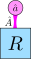
\includegraphics[width=0.2\linewidth, draft=false]{phog/single_mode}
\caption{\label{fig:phog_single_mode} A single bosonic mode, $a$, is coupled to a Markovian reservoir $R$ by operator $\hat{A}$. }
\end{figure}

\MT{Make sure that my analysis in this section is sufficiently motivated and doesn't seem like too much of a detour.}

Consider the model displayed in Fig.~\ref{fig:phog_single_mode} (c.f. Fig.~\ref{fig:phog_models}\MakeUppercase{\romannumeral 1}), which consists of a single bosonic mode, $a$, coupled to a reservoir $R$ via a reservoir operator $\mathcal{A}$. The annihilation (creation) operator for mode $a$ is denoted $\hat{a} \left(\hat{a}^\dagger\right)$, and the density matrix containing all information about the state of the mode is denoted $\rho_a$. This model will prove illustrative of several principles which we will develop throughout the chapter. Assuming that reservoir $R$ is Markovian, the evolution of mode $a$ is given by the following quantum master equation in Lindblad form\footnote{Equations in this form will be referred to as ``Lindblad equations''}

\begin{equation}\label{eqn:phog_lindblad_1}
\ddt \rho_a =  - i \left[\hat{H}, \rho_a\right] + \gamma \mathcal{L}\left(\hat{A}\right)\rho_a
\end{equation}

\noindent In what follows we consider the case with Hamiltonian $\hat{H} = \hbar \omega \hat{a}^\dagger \hat{a}$. Eq.~\ref{eqn:phog_lindblad_1} then describes the decay of state $\rho_a\left(t=0\right)$ into $R$ with rate $\gamma$. The Lindbladian term $\mathcal{L}\left(\hat{A}\right)$ takes the usual form
\begin{equation}\label{eqn:phog_lindbladian_form}
\mathcal{L}\left(\hat{A}\right)\rho_a = \hat{A}\rho_a\hat{A}^\dagger - \frac{1}{2} \hat{A}^\dagger \hat{A} \rho_a - \frac{1}{2} \rho_a \hat{A}^\dagger \hat{A}.
\end{equation}

\noindent Let us consider the behaviour of an initially coherent state $\rho_a\left(t=0\right) = \dyad{\alpha}$ with amplitude $\alpha$. We will explore several choices for decay operator $\hat{A}$.

\subsection{$\hat{A} = \hat{a}$}
First, we will explore the case where the decay into the reservoir is governed by mode $a$ annihilation operator, $\hat{a}$, which corresponds to single-photon loss.% I can refer to intro chapter for properties of this.
The evolution of $\rho_a$ is described by

\begin{equation}\label{eqn:phog_lindblad_single_photon_loss}
\ddt \rho_a = \gamma\left[\hat{a}\rho_a \hat{a}^\dagger - \frac{1}{2} \hat{a}^\dagger \hat{a} \rho_a - \frac{1}{2} \rho_a \hat{a}^\dagger \hat{a}\right],
\end{equation}
where we have transformed into a rotating frame and so the free Hamiltonian term $\hbar \omega \hat{a}^\dagger \hat{a}$ vanishes. Let us calculate the evolution $\langle \hat{a}^\dagger \hat{a}\rangle\left(t\right)$ of photon number expectation:

\begin{align}
\ddt \langle \hat{a}^\dagger \hat{a}\rangle &= \gamma \left[ \text{Tr}\left(\hat{a}^\dagger \hat{a} \hat{a} \rho_a \hat{a}^\dagger \right) - \frac{1}{2} \text{Tr}\left(\hat{a}^\dagger \hat{a} \hat{a}^\dagger \hat{a} \rho_a\right) - \frac{1}{2} \text{Tr}\left(\hat{a}^\dagger \hat{a} \rho_a \hat{a}^\dagger \hat{a}\right)\right] \notag \\
%
&= \gamma \left[ \langle \hat{a}^\dagger \hat{a}^\dagger \hat{a}\hat{a}\rangle - \langle \hat{a}^\dagger \hat{a} \hat{a}^\dagger \hat{a}\rangle \right] \notag \\
%
&= - \gamma \langle \hat{a}^\dagger \hat{a}\rangle
\end{align}
\noindent and so
\begin{equation}
\langle\hat{a}^\dagger \hat{a} \rangle \left(t\right) = \langle \hat{a}^\dagger \hat{a}\rangle \left(0\right) e^{- \gamma t}
\end{equation}
the photon number exponentially decays in time with decay rate $\gamma$. We may derive similar equations for $\langle\hat{x}\rangle\left(t\right)$ and $\langle\hat{x}\rangle\left(t\right)$ and find 
\begin{align}
\ddt \langle \hat{x}\rangle &= \langle \hat{x}\rangle\left(0\right) e^{- \frac{\gamma}{2} t} \notag \\
%
\ddt \langle \hat{p}\rangle &= \langle \hat{p}\rangle \left(0\right) e^{- \frac{\gamma}{2} t}.
\end{align}

\noindent We might guess that the steady-state of Eq.~\ref{eqn:phog_lindblad_single_photon_loss} is the vacuum $\dyad{0}$, and indeed we can deduce that this must be the case by noticing that $\ddt \rho_a = 0$ when $\rho_a$ is vacuum. In Fig.~\ref{fig:phog_lindblad_single_photon_loss} we plot the evolution of $\langle\hat{a}^\dagger \hat{a}\rangle, \langle \hat{x}\rangle, \langle \hat{p}\rangle$ and the fidelities between $\rho_a\left(t\right)$ and the vacuum steady state, and between $\rho_a\left(t\right)$ and a coherent state with photon expectation $\langle\hat{a}^\dagger \hat{a}\rangle\left(t\right)$. We additionally plot the time-evolution of quadrature variances $\langle \text{Var}\left(\hat{x}\right)\rangle$ and $\langle \text{Var}\left(\hat{p}\right)\rangle$, and we see that they remain constant. \MT{TODO: plot the things}

\begin{figure}[htp]
\centering
\includegraphics{phog/phog_lindblad_single_photon_loss.png}
\caption{\label{fig:phog_lindblad_single_photon_loss}}
\end{figure}

\subsection{$\hat{A} = \hat{a}^2$}
Next we consider a two-photon loss term $\hat{a}^2$, which describes two-photon decay into the reservoir. Our Lindblad equation is

\begin{equation}\label{eqn:phog_lindblad_two_photon_loss}
\ddt \rho_a = \gamma\left[\hat{a}^2 \rho_a \hat{a}^{\dagger 2} - \frac{1}{2} \hat{a}^{\dagger 2} \hat{a}^2 \rho_a - \frac{1}{2} \rho \hat{a}^{\dagger 2} \hat{a}^2\right]
\end{equation}
which gives the evolution of photon number expectation as 
\begin{equation}
\ddt \langle \hat{a}^\dagger \hat{a}\rangle = - 2 \gamma \langle \hat{a}^\dagger \hat{a}^\dagger \hat{a}\hat{a}\rangle
\end{equation}
which does not take a closed form and so we cannot yet directly calculate $\langle \hat{a}^\dagger \hat{a}\rangle\left(t\right)$. Similarly, equations for evolution of $\langle\hat{a}\rangle\left(t\right)$ require terms to the third power in the creation/annihilation operators, and so are not yet closed.  We will see techniques in Sec.~\ref{sec:linearization} which allow us to deal with this.

For now, let us deduce what must be the steady-state of Eq.~\ref{eqn:phog_lindblad_two_photon_loss}. We observe that once again the vacuum $\dyad{0}$ must be a steady state, since then $\ddt \rho_a=0$. Surprisingly we now also have the single-photon state $\dyad{1}$ as a steady state since this also has $\ddt \rho_a=0$. The general steady-state is a superposition of these
\begin{equation}\label{eqn:phog_phase_state}
\ket{\psi} = \ket{0} + e^{i \phi} \ket{1} \qq{with} \rho_a\left(t \rightarrow \infty\right) = \dyad{\psi}
\end{equation}
which takes the form of a so-called \emph{phase state}, and has long been known that the steady state of two-photon loss is a phase-state. The phase $\phi$ is related to the phase of the initial coherent state. \MT{show this.}
\MT{check how the state is normalized}

In Fig.~\ref{fig:phog_lindblad_two_photon_loss} we plot the evolution of $\langle \hat{a}^\dagger \hat{a}\rangle, \langle \hat{x}\rangle, \langle \hat{p}\rangle$ and the fidelities between $\rho_a\left(t\right)$ and the final phase state, and between $\rho_a\left(t\right)$ and a coherent state with the same photon expectation as $\rho_a\left(t\right)$. We also show the time-evolution of quadrature variances. \MT{TODO: do this}

\begin{figure}[htp]
\centering
\includegraphics{phog/phog_lindblad_two_photon_loss.png}
\caption{\label{fig:phog_lindblad_two_photon_loss}}
\end{figure}

\MT{TODO: analytically show in fock basis the steady state.}

\subsection{$\hat{A} = \hat{a}^3$}
We might guess that the steady state of the three-photon loss term $\hat{a}^3$ is likewise a superposition of $\ket{0}, \ket{1}$ and $\ket{2}$
\begin{equation}
\rho_a\left(t\rightarrow\infty\right) \stackrel{?}{=} \ket{0} + e^{i \phi}\ket{1} + e^{i \varphi}\ket{2}
\end{equation}
\MT{check how the state is normalized}
with phases $\phi, \varphi$ in general depending on the initial coherent state $\dyad{\alpha}$. \MT{TODO: investigate this numerically}

\MT{TODO: analytically show in fock basis the steady state}

\subsection{$\hat{A} = \hat{a}\left(\hat{a}^\dagger \hat{a} - 1\right)$}
We have seen that the choice of $\hat{A}$ can give drastically different steady states of $\rho_a$,  from the uninteresting vacuum to the highly quantum and useful phase-state. We therefore wish to consider which choices for $\hat{A}$ will give rise to the highly desired Fock states.

The choice 
\begin{equation}\label{eqn:phog_A_ncl}
\hat{A} = \hat{a}\left(\hat{a}^\dagger \hat{a} - 1\right)
\end{equation}
may be interpreted as a single-photon loss with a rate which depends on photon number. We should be able to see that the rate goes to zero for the state $\dyad{1}$. Therefore, the single-photon state $\dyad{1}$ is a steady state of this loss mechanism. 

The vacuum state $\dyad{0}$ also happens to be a steady-state of $\ncl$, but \MT{its coefficient remains constant, so we obtain $\dyad{1}$ in the limit of $\alpha\rightarrow \infty$}

\MT{TODO: analytically show in fock basis the steady state and everything}

Let us examine the evolution of $\rho_a$. In Fig.~\ref{fig:phog_A_ncl} we plot the evolution of photon number, $\langle \hat{x}\rangle, \langle \hat{p}\rangle$ and fidelities between $\rho_a\left(t\right)$ and $\dyad{1}$, and between $\rho_a\left(t\right)$ and a coherent state with equivalent photon number. We also plot the time-evolution of the quadrature variances.

\begin{figure}[htp]
\centering
\includegraphics{phog/phog_A_ncl.png}
\caption{\label{fig:phog_A_ncl}}
\end{figure}

\subsection{$\hat{A} = \hat{a} \left(\hat{a}^\dagger \hat{a} - 2\right)$}
Similarly, let us explore the evolution of $\rho_a$ under loss operator $\hat{a} \left(\hat{a}^\dagger \hat{a} - 2\right)$. By the same arguments as above, we might reasonably expect the steady state to be a weighted superposition of $\ket{0}, \ket{1}$ and $\ket{2}$ with the coefficients of $\ket{0}, \ket{1}$ taking their initial values. Therefore in the limit $\alpha\rightarrow\infty$ we expect the steady state to be the two-photon Fock state $\dyad{2}$, and this is indeed what we see, Fig.~\ref{fig:phog_A_ncl2}.

\begin{figure}[htp]
\centering
\includegraphics{phog/phog_A_ncl2.png}
\caption{\label{fig:phog_A_ncl2}}
\end{figure}

\MT{Gotta create all these figures and then interpret them.}

\section{Including loss}
We have seen that the loss operator $\ncl$ is a good canditate for driving an initial coherent state towards a single photon state $\ket{1}$. Any system, therefore, which can implement the Lindblad equation~\ref{eqn:phog_lindblad_1} with $\hat{A} = \ncl$ will asymptotically give rise to single-photon Fock states. 

